\chapter{About the Author}
\pagestyle{empty}
\begin{wrapfigure}{R}{0.4\textwidth}
\centering
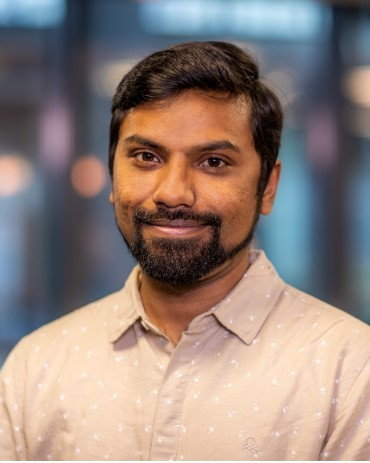
\includegraphics[width=0.35\textwidth]{Figures/sajid.jpg}
\end{wrapfigure}

% \begin{sloppypar}
Sajid Mohamed was born on July 6, 1990 in Trivandrum, Kerala, India. 
He studied at the National Institute of Technology (NIT) Calicut, where he obtained the Bachelor of Technology (B.Tech.) degree in Electrical \& Electronics Engineering in 2012.
He obtained his Master of Technology (M.Tech.) degree in Embedded Controls \& Software in 2014 from the Indian Institute of Technology (IIT) Kharagpur.
He was awarded the German Academic Exchange Service (DAAD) scholarship to pursue his Master's thesis
on Timed Abstractions and Analysis of Distributed Real-Time Control Architectures
at the Technical University of Munich (TUM) in the Institute for Real-Time Computer Systems.
He was a research assistant at IIT Kharagpur from 2014 to 2016.

In 2016, Sajid was awarded the Marie Skłodowska-Curie Scholarship and joined the Electronic Systems group of Eindhoven University of Technology (TU/e) as an Early-Stage Researcher in the \emph{Platform-aware Model-driven Optimization of Cyber-Physical Systems (oCPS)} project.
The project focused on training a generation of young researchers in cross-disciplinary thinking and delivering industrially validated toolchains by bringing together the state of the practice through six key industrial players and the state-of-the-art through four top universities and one research institute across Europe.
In 2020, Sajid continued working in TU/e as a University Researcher in the FitOptiVis project.
The results of his research have led, among others, to several peer-reviewed publications and the contents of this dissertation.
In July 2021, he started his current job as a Principal Software Engineer in the Innovation Team of ITEC B.V.
% \end{sloppypar}